\documentclass[../../main.tex]{subfiles}
\graphicspath{{../../image/}{../../figure/}}
\begin{document}

\section{标量守恒律的前沿追踪}\label{section:ch14-标量守恒律的前沿追踪}

本节讨论通过一种旨在消除稀疏波的前沿追踪格式构造标量守恒律初值问题的可容许解。其建筑砌块将是由常状态、可容许``压缩性''激波与不可容许``稀疏性''小强度激波组成的复合波。

通量 $f\in C^1$ 的标量守恒律 $\partial_t u+\partial_x f(u)=0$ 的 Riemann 问题可容许解已在\cref{section:ch09-一般严格双曲方程组}中构造：左端状态 $u_l$ 与右端状态 $u_r$ 由波扇
\begin{align}
u(x,t)=[g']^{-1}\!\left(\frac{x}{t}\right),
\label{align:ch14-scalar-riemann}
\end{align}
相连接，其中当 $u_l<u_r$ 时 $g$ 是 $f$ 在 $[u_l,u_r]$ 上的凸包，当 $u_l>u_r$ 时 $g$ 是 $f$ 在 $[u_r,u_l]$ 上的凹包。$g'$ 为常数的区间产生激波，而 $g'$ 严格单调的区间产生稀疏波。即使 $f$ 仅是 Lipschitz 连续，同一构造仍然适用，只是此时复合波中除激波与稀疏波外还可能含有中间常状态，即 $g'$ 的跳跃点。特别地，当 $f$（从而 $g$）是分段线性时，复合波不含任何稀疏波，而仅由激波与常状态组成（见\cref{figure:ch14-标量riemann复合波}）。

\begin{figure}[ht]
\centering
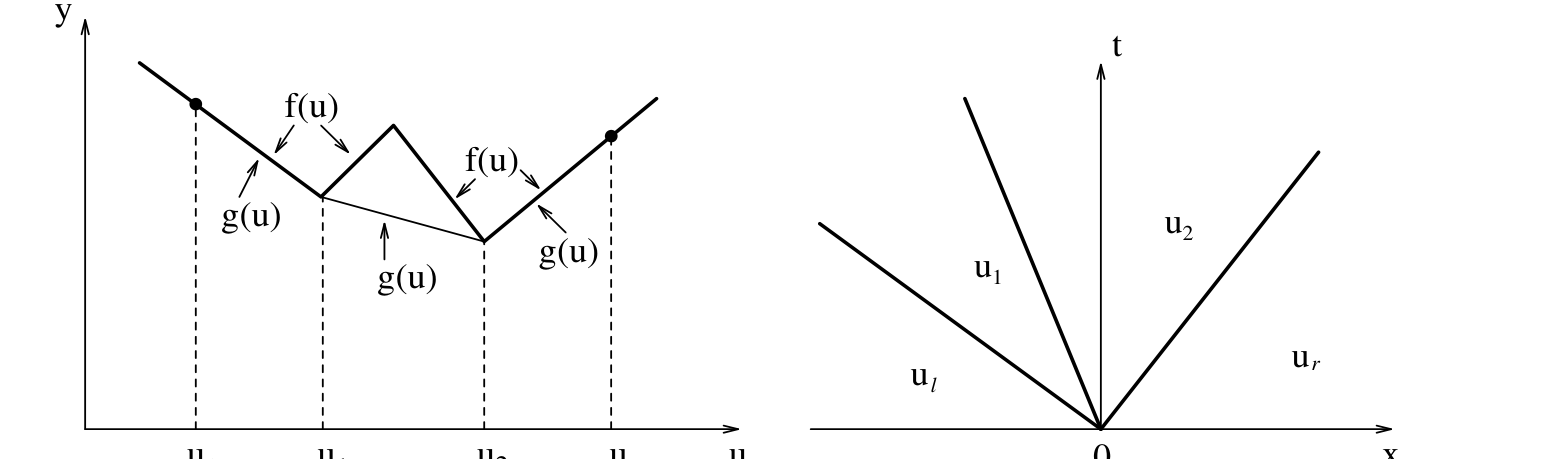
\includegraphics[width=0.9\textwidth]{ch14-fig01-01.png}
\caption{凸包/凹包与相应的复合波扇}\label{figure:ch14-标量riemann复合波}
\end{figure}

现考虑 Cauchy 问题
\begin{align}
\begin{cases}
\partial_t u(x,t)+\partial_x f(u(x,t))=0, & -\infty<x<\infty,\ 0\leqslant t<\infty,\\
u(x,0)=u_0(x), & -\infty<x<\infty,
\end{cases}
\label{align:ch14-scalar-cauchy}
\end{align}
其中通量 $f$ 在 $(-\infty,\infty)$ 上 Lipschitz 连续，初值 $u_0$ 取值于有界区间 $[-M,M]$ 且在 $(-\infty,\infty)$ 上有有界总变差。

为求解\eqref{align:ch14-scalar-cauchy}，先用一列分段线性函数 $\{f_m\}$ 逼近通量 $f$，使 $f_m$ 的图像是内接于 $f$ 图像的折线，顶点位于点 $\left(\frac{k}{m},f\!\left(\frac{k}{m}\right)\right)$，$k\in\mathbb{Z}$。接着，把初值 $u_0$ 实现为一列阶梯函数 $\{u_{0m}\}$ 的 a.e. 极限，其中 $u_{0m}$ 取值于集合 $\mathscr{U}_m=\left\{\frac{k}{m}:k\in\mathbb{Z},\ |k|\leqslant mM\right\}$，且其总变差不超过 $u_0$ 在 $(-\infty,\infty)$ 上的总变差。最后，对 $m=1,2,\cdots$ 求解初值问题
\begin{align}
\begin{cases}
\partial_t u(x,t)+\partial_x f_m(u(x,t))=0, & -\infty<x<\infty,\ 0\leqslant t<\infty,\\
u(x,0)=u_{0m}(x), & -\infty<x<\infty,
\end{cases}
\label{align:ch14-scalar-approx}
\end{align}
目标是证明：\eqref{align:ch14-scalar-approx}的可容许解 $u_m$ 是取值于 $\mathscr{U}_m$ 的分段常值函数，它通过求解守恒律\eqref{align:ch14-scalar-approx}$_1$的有限多个 Riemann 问题而构造；并且序列 $\{u_m\}$ 收敛到\eqref{align:ch14-scalar-cauchy}的可容许解 $u$。

$u_m$ 的构造始于求解 Riemann 问题，把 $u_{0m}$ 的跳跃间断分解为 $\mathscr{U}_m$ 中的激波与常状态。继而，由激波碰撞诱发的波相互作用按其发生顺序类似地分解为 $\mathscr{U}_m$ 中的激波与常状态，它们由 Riemann 问题的解产生。应当注意：端状态属于 $\mathscr{U}_m$ 的\eqref{align:ch14-scalar-approx}$_1$ 的 Riemann 问题可容许解也是\eqref{align:ch14-scalar-cauchy}$_1$ 的解，尽管在该情形下它未必是可容许解，因为某些跳跃间断可能是稀疏激波。因而 $u_m$ 除是\eqref{align:ch14-scalar-approx}的可容许解外，还是\eqref{align:ch14-scalar-cauchy}$_1$ 的一个（一般不可容许）解。

我们证明：在上述算法的执行中可能遇到的激波碰撞次数是先验有界的，从而 $u_m$ 在整个上半平面上经有限步构造完成。其原因在于：每次激波相互作用都通过降低激波数目或``振荡''数目来简化波型。激波数目由阶梯函数 $u_m(\cdot,t)$ 的跳跃间断点数 $j_m(t)$ 度量；``振荡''数目由 $u_m(\cdot,t)$ 的环绕数 $\ell_m(t)$ 计数，其定义如下。

对 $(-\infty,\infty)$ 上的阶梯函数 $v(\cdot)$，当 $v(\cdot)$ 单调时令环绕数 $\ell=0$；当 $v(\cdot)$ 非单调时，把 $\ell$ 定义为最大正整数，使得存在 $\ell+2$ 个 $v(\cdot)$ 的连续点 $-\infty<x_0<\cdots<x_{\ell+1}<\infty$，满足 $[v(x_{i+1})-v(x_i)][v(x_i)-v(x_{i-1})]<0$，$i=1,\cdots,\ell$。

显然，$j_m(t)$ 与 $\ell_m(t)$ 在相邻激波碰撞之间的开时间区间上保持常数；它们仅在 $t=0$ 处以及激波碰撞时改变。当 $k$ 个连接（左、右）状态 $(u_0,u_1),\cdots,(u_{k-1},u_k)$ 的激波在一点碰撞时，若有限序列 $\{u_0,u_1,\cdots,u_k\}$ 单调，则称所产生的相互作用为单调的。此种相互作用产生单个激波，左端为状态 $u_0$、右端为状态 $u_k$。特别地，单调相互作用保持 $\ell_m(t)$ 不变，而使 $j_m(t)$ 至少下降 1。相反，跨非单调相互作用时 $\ell_m(t)$ 至少下降 1，而 $j_m(t)$ 可朝任一方向变化，但无论如何其增加量不超过 $s_m-1$，其中 $s_m$ 是 $f_m'$ 在区间 $(-M,M)$ 上的跳跃点数；于是 $s_m-1<2Mm$。由此，整值函数
\begin{align*}
p_m(t)=j_m(t)+s_m\ell_m(t)
\end{align*}
在相邻激波碰撞之间的开时间区间上保持常数，而跨任一单调或非单调激波碰撞时至少下降 1。跨 $t=0$ 轴，有 $\ell_m(0+)=\ell_m(0)$ 与 $j_m(0+)\leqslant(s_m+1)j_m(0)$。因此 $(s_m+1)[j_m(0)+\ell_m(0)]$ 给出 $u_m$ 构造中所涉及激波碰撞总数的上界。

作为 $t$ 的函数，$u_m(\cdot,t)$ 在 $(-\infty,\infty)$ 上的总变差在相邻激波碰撞之间的时间区间上保持常数；跨单调激波碰撞时不变；跨非单调激波碰撞时下降。因而
\begin{align}
TV_{(-\infty,\infty)}u_m(\cdot,t)\leqslant TV_{(-\infty,\infty)}u_m(\cdot)\leqslant TV_{(-\infty,\infty)}u_0(\cdot),\qquad 0\leqslant t<\infty.
\label{align:ch14-scalar-tv}
\end{align}
由于 $u_m$ 的任一激波速度不超过 $f$ 在 $[-M,M]$ 上的 Lipschitz 常数 $c$，\eqref{align:ch14-scalar-tv}蕴含
\begin{align}
\int_{-\infty}^{\infty}|u_m(x,t)-u_m(x,\tau)|\,\mathrm{d}x\leqslant c|t-\tau|\,TV_{(-\infty,\infty)}u_0(\cdot),\qquad 0\leqslant\tau<t<\infty.
\label{align:ch14-scalar-lip}
\end{align}
借助\eqref{align:ch14-scalar-tv}、Helly 定理与 Cantor 对角线过程，可取子列 $\{u_{m_k}\}$，使对任一有理数 $t\in[0,\infty)$，$\{u_{m_k}(\cdot,t)\}$ 在 $L^1_{\mathrm{loc}}(-\infty,\infty)$ 中收敛。于是\eqref{align:ch14-scalar-lip}蕴含对所有 $t\in[0,\infty)$，$\{u_{m_k}(\cdot,t)\}$ 是 $L^1_{\mathrm{loc}}(-\infty,\infty)$ 中的 Cauchy 列，从而 $\{u_{m_k}\}$ 在 $L^1_{\mathrm{loc}}$ 中收敛到某个在 $(-\infty,\infty)\times[0,\infty)$ 上局部有界变差的函数 $u$。

如\cref{chapter:ch06-标量守恒律L1理论}所讨论，由于 $u_m$ 是\eqref{align:ch14-scalar-approx}的可容许解，
\begin{align}
\int_0^\infty\int_{-\infty}^\infty[\partial_t\psi\eta(u_m)+\partial_x\psi q_m(u_m)]\,\mathrm{d}x\,\mathrm{d}t+\int_{-\infty}^\infty\psi(x,0)\eta(u_{0m}(x))\,\mathrm{d}x\geqslant 0,
\label{align:ch14-scalar-entropy}
\end{align}
对任一凸熵 $\eta$（其相应熵流 $q_m=\int\eta'\,\mathrm{d}f_m$）以及所有 $(-\infty,\infty)\times[0,\infty)$ 上具有紧支集的非负 Lipschitz 检验函数 $\psi$ 成立。当 $m\to\infty$ 时，$\{u_{0m}\}$ 在 $(-\infty,\infty)$ 上 a.e. 收敛到 $u_0$，$\{q_m\}$ 在 $[-M,M]$ 上一致收敛到函数 $q=\int\eta'\,\mathrm{d}f$，即守恒律\eqref{align:ch14-scalar-cauchy}$_1$ 中与熵 $\eta$ 相应的熵流。沿子列 $\{m_k\}$ 在\eqref{align:ch14-scalar-entropy}中取极限，我们推得
\begin{align}
\int_0^\infty\int_{-\infty}^\infty[\partial_t\psi\eta(u)+\partial_x\psi q(u)]\,\mathrm{d}x\,\mathrm{d}t+\int_{-\infty}^\infty\psi(x,0)\eta(u_0(x))\,\mathrm{d}x\geqslant 0,
\label{align:ch14-scalar-entropy-limit}
\end{align}
后者转而蕴含 $u$ 是\eqref{align:ch14-scalar-cauchy}的可容许解。由唯一性，我们推断整个序列 $\{u_m\}$ 收敛到 $u$。

\end{document}
